\documentclass[a4paper, 12pt]{article}
\usepackage[T2A]{fontenc}
\usepackage[utf8]{inputenc}
\usepackage[english,russian]{babel}
\usepackage{amsmath, amsfonts, amssymb, amsthm, mathtools, misccorr, indentfirst, multirow}
\usepackage{wrapfig}
\usepackage{graphicx}
\usepackage{subfig}
\usepackage{adjustbox}
\usepackage{pgfplots}

\usepackage{geometry}
\geometry{top=20mm}
\geometry{bottom=20mm}
\geometry{left=20mm}
\geometry{right=20mm}
\newcommand{\angstrom}{\textup{\AA}}
\begin{document}
	\begin{titlepage}
		\begin{center}
		МИНИСТЕРСТВО ОБРАЗОВАНИЯ И НАУКИ РОССИЙСКОЙ ФЕДЕРАЦИИ\\
		\footnotesize{Московский физико-технический институт}\\
		\footnotesize{(государственный университет)}\\
		\footnotesize{Кафедра вакуумной электроники}\\
		\vfill
		{\LARGE
		\textbf{Атомно силовой микроскоп}\\
		}
		\vspace{1cm}
		Лабораторная работа по курсу\\
		вакуумная электроника
		\vfill
		\begin{flushright}
			Выполнил: студент 654гр.\\
			Нехаев А.С.
		\end{flushright}
		\vfill
		г. Долгопрудный\\
		2018 год
		\end{center}
	\end{titlepage}
	\newpage
	\pagenumbering{arabic}
	\tableofcontents
	\newpage
	\section{Цель работы}
	Ознакомиться на практике с физическими принципами функционирования атомно-силового микроскопа и основными методиками измерения.\par
	Изучить работу сканирующего зондового микроскопа NanoEducator, проведя измерения в бесконтактном атомно-силовом режиме.\par
	\newpage
	\section{Практическая часть}
	\subsection{Измерение резонансной частоты собственных колебаний кантилевера}
	В атомно силовом микроскопе используются зонды кантилеверного типа. Кантилевер представляет собой балку, один конец которой закреплен на твердой подложке, которая вставляется в держатель зонда, расположенного под сканером. Второй конец кантилевера свободен и на нем находится острая игла.\par
	Важными характеристиками кантилевера являются коэффициент жесткости и резонансная частота материала. Первый должен быть минимально низкий, чтобы кантилевер мог изгибаться под действием сверхмалых сил, вторая же при этом должна быть максимально высокой, чтобы в игле не возбуждались собственные колебания возвратно-поступательных движений.\par
	Проведем измерения АЧХ зонда для определения резонансной частоты материала кантилевера.\par
	\begin{figure}[!htb]
		\includegraphics[width=\textwidth]{ach1.PNG}
		\caption{Амплитудно-частотная характеристика зонда}
	\end{figure}
	Данные показатели для различных кантилеверов определяются геометрическими размерами и материалом изготовления и лежат в интервале от 0.01 до 100 Н/м для коэффициента упругости и 15-500 кГц для резонансной частоты собственных колебаний.\par
	Как видно из графика АЧХ зонда, резонансная частота собственных колебаний кантилевера равна 8.15 кГц, что в полтора раза меньше нижней границы, заявленной в теоретических данных.\par
	\subsection{Разрешающая способность микроскопа в контактном режиме}
	Критерием разрешающей способности по нормали $\Delta Z$ может служить минимальное изменение координаты $Z$ при сканировании, детектируемое на уровне шумов.\par
	Пусть зондирующее острие характеризуется радиусом кривизны $R$, разрешаемые особенности поверхности $r$, тогда возможность \textit{латерального} разрешения поверхностных особенностей $d$ будет связана с пределом разрешения по нормали $\Delta Z$. Критерием разрешения является условие возможности детектирования разницы в значениях вертикальной координаты иглы над объектами и между ними.\par
	Соотношение минимального расстояния между разрешаемыми поверхностными особенностями, при котором <<провал>> между ними на АСМ-изображении ещё может быть детектирован (равен пределу $\Delta Z$):
	\begin{equation*}
		d\approx\sqrt{8(R+r)\Delta Z}
	\end{equation*}
	\par
	Поскольку достижимое пространственное разрешение должно являться инвариантом, то его следует определить, рассматривая условия детектирования двух точечных объектов ($r = 0)$, тогда:
	\begin{equation*}
		d=\sqrt{8R\Delta Z}
	\end{equation*}
	\par
	Таким образом, связав разрешения латеральное $d$ и по нормали $\Delta Z$, можно найти радиус кривизны зондирующего острия $R$.
	\begin{figure}[!htb]
		\centering
		\includegraphics[scale=0.7]{20.11.2018/topview1.jpg}
		\caption{Топография решетки}
		\label{pic1}
	\end{figure}
	\newpage
	\begin{figure}[!htb]
		\centering
		\includegraphics[scale=0.6]{relief1.jpg}
		\caption{Вертикальное сечение выступа, изображенного на рис. \ref{pic1}}
	\end{figure}
	Полученное вертикальное сечение позволяет оценить радиус кривизны острия зонда:
	\begin{equation*}
		R=\frac{d^2}{8\Delta Z}=2.8\ \text{мкм}
	\end{equation*}
	\begin{figure}[!htb]
		\centering
		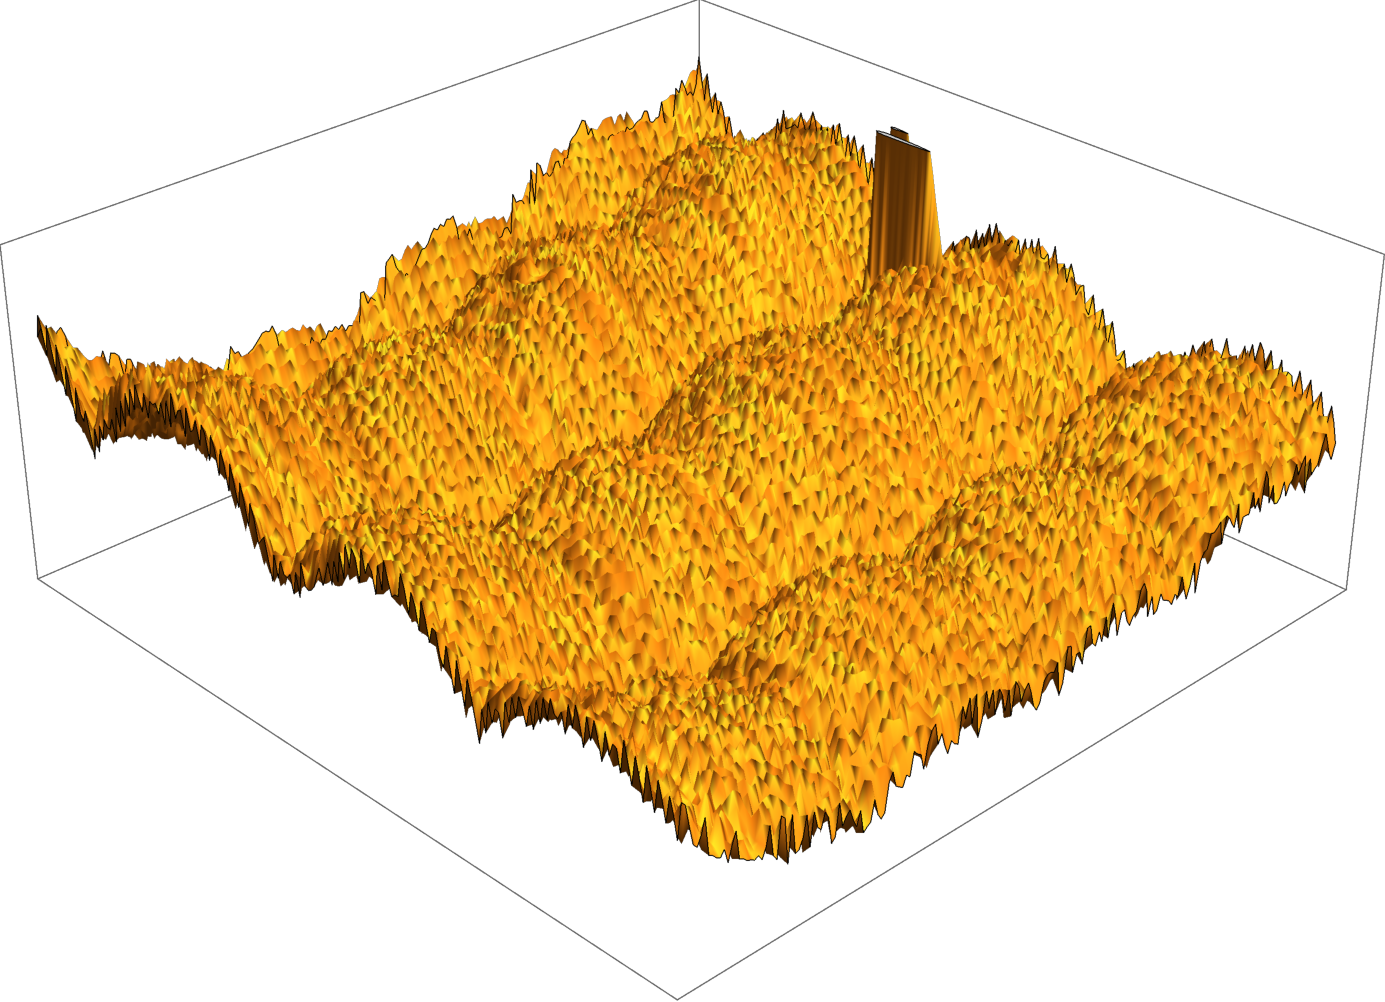
\includegraphics[scale=0.6]{3d.pdf}
		\caption{Трехмерное изображение рельефа}
	\end{figure}
	\subsection{Бесконтактный режим работы прибора}
	В микроскопе NanoEducator в качестве основного режима сканирования используется \textit{бесконтактный} режим. В этом режиме работы зонд находится достаточно близко от поверхности образца в области действия сил притяжения.\par
	Силы притяжения и их градиенты обычно слабее отталкивающих контактных сил, поэтому для их детектирования обычно используется модуляционная методика. Для этого \textit{пьезовибратор}, на котором укреплен кантилевер с зондом прикладывается переменное напряжение, которое вызывает изменение его геометрических размеров.
	\begin{figure}[!htb]
		\centering
		\includegraphics[scale=0.7]{spectr1.PNG}
		\caption{Кривая спектроскопии}
	\end{figure}
	\par
	\paragraph{Спектроскопия.} Пьезодрайвер программируется таким образом, чтобы компенсировать отталкивающие контактные силы для выражения более слабых гравитационных сил и их детектирования. Для этого производится калибровка корректирующего сигнала пьезодрайвера $\omega$ по расстоянию зонд-образец $z$.\par
	Уравнение, описывающее движение зонда при малой амплитуде колебаний:
	\begin{equation*}
		\frac{d^2z}{dt^2}+\frac{\omega_0}{Q}\frac{dz}{dt}+\omega_0^2(z-z_0)=\Delta z\omega_0^2\cos(\omega t)
	\end{equation*}
	Сдвиг фаз $\varphi$ колебаний свободного конца кантилевера относительно закрепленного определяется выражением:
	\begin{equation*}
		\tan\varphi=\frac{1}{Q}\frac{\omega\omega_0}{\omega_0^2-\omega^2}
	\end{equation*}
	\par
	Приближение зонда к поверхности образца приводит к возникновению заметного градиента силы взаимодействия между ними., что приводит к смещению АЧХ и ФЧХ колебаний кантилевера влево по сравнению с измеренными вдали от поверхности.\par
	Резонансная частота изменяется при изменении градиента силы $\delta F/\delta z$ (при приближении зонда к поверхности) по сравнению со свободно резонирующим кантилевером (вдали от поверхности) в соответствие с выражением:
	\begin{equation*}
		\overline{\omega}=\omega_0\sqrt{1-\frac{1}{k}\frac{\delta F}{\delta z}}
	\end{equation*}
	\par
	Так как частота вынуждающих колебаний кантилевера поддерживается постоянной и равной $\omega_0$ в свободном состоянии, то при приближении зонда к поверхности образца амплитуда регулируется с помощью оптической системы и может быть определена по относительному изменению переменной освещенности верхней и нижней половинок фотодетектора. Далее с помощью синхронного детектора выделяется постоянный сигнал, согласованный с синхросигналом от генератора напряжений.\par
	Компаратор сохраняет текущий сигнал в цепи сенсора с изначально заданным напряжением $V_s$ (характеризует уровень силы, на котором зонд удерживается от поверхности образца) и при его отклонении вырабатывает корректирующий сигнал $V_{fb}$. Взаимодействие зонда и образца поддерживается постоянным за счет приближения и отвода системы обратной связи, управляющей $Z$-пьезоприводом таким образом, чтобы сила взаимодействия между зондом и образцом была постоянной. Сигнал о высоте $z$ берется в каждой точке плоскости изображения $(x,y)$ из канала $Z$-пьезопривода.\par
	В результате спектроскопии было обнаружено, что для поддерживания взаимодействия зонда с образцом на расстоянии $z = 0$ постоянным требуется корректирующий сигнал, равный $V_{fb}=0.07 V_s$
	\section{Вывод}
	В ходе работы мы ознакомились на практике с физическими принципами функционирования атомно-силового микроскопа и основными методиками измерения.\par
	Изучили работу сканирующего зондового микроскопа NanoEducator.\par
	Оценили радиус кривизны острия зонда по разрешающей способности АСМ в контактном режиме для решётки (2.8 мкм).\par
	Определили при помощи спектроскопии величину корректирующего сигнала для поддерживания взаимодействия зонда с образцом на расстоянии $z = 0$ постоянным $(V_{fb} = 0.07V_s)$.
\end{document}